\documentclass[12pt]{article}

\usepackage{times}
\usepackage{graphicx}
\usepackage{amsmath}
\usepackage{url}
\usepackage{algorithmic}
\usepackage{enumerate}

\setlength{\textwidth}{6.5in}
\setlength{\textheight}{8.9in}
\setlength{\oddsidemargin}{0.0in}
\setlength{\topmargin}{0.05in}
\setlength{\headheight}{-0.05in}
\setlength{\headsep}{0.0in}

\begin{document}

\begin{center}
{\bf CS 6300} \hfill {\large\bf HW10: Particle Filters and POMDPs \hfill Due April 26, 2022}
\end{center}

\noindent
Please use the \LaTeX\ template to produce your writeups.  Hand in via
gradescope.

\section{Particle Filtering}
  
A garbage-collecting robot lives in a 4x4 Manhattan grid city.  The
associated HMM includes the robot position $X$, the readings $G$ from
a garbage sensor, and ($A$,$B$,$C$,$D$) readings from the motion
sensors.

\begin{figure}[h]
\centering{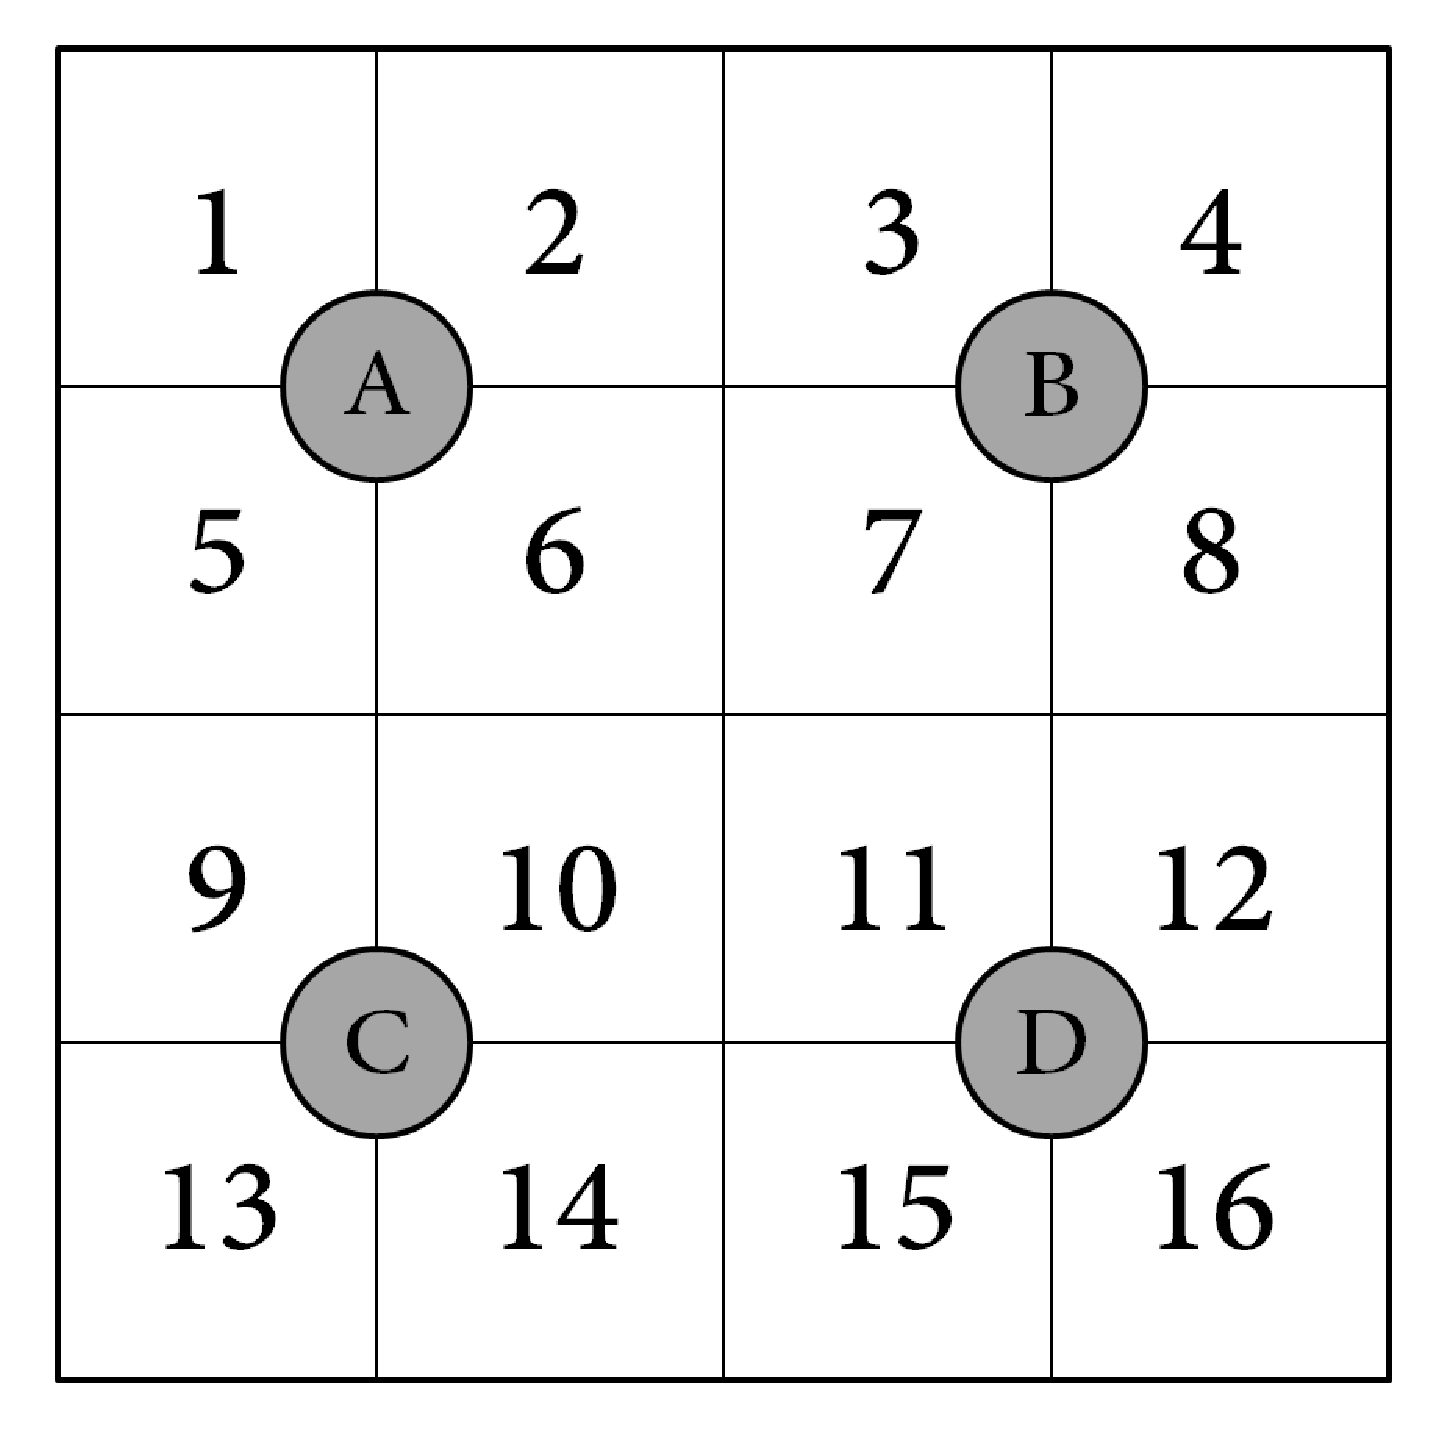
\includegraphics[scale=.19]{particle_filter_grid.eps} \hspace{1cm}
 \includegraphics[scale=.2]{particle_filter_hmm.eps} \hfill}
\end{figure}
  
The garbage sensor $G$ takes on an integer value between 1 and 16,
corresponding to the square with the most garbage at time $t$.  The
robot is programmed to move toward the square with the most garbage,
but it will only take an optimal action with probability 0.9.  In each
time step, the robot can either stay in the same square, or move to an
adjacent square. In case where multiple actions would move it equally
close to the desired position, the robot has an equal probability of
taking any of these actions. In case the robot fails to take an
optimal action, it has an equal probability of taking any of the
non-optimal actions. For example, if the robot is in square 2, the
actions available are (EAST, SOUTH, WEST, STOP). If $G_t = 15$, the
transition model will look like this:

\begin{center}
\renewcommand{\arraystretch}{1.2}
\begin{tabular} {|c|c|}
\hline
$X_{t+1}$ & $P(X_{t+1}|X_t=2,G_t=15)$ \\
\hline
1 & 0.05 \\
2 & 0.05 \\
3 & 0.45 \\
6 & 0.45 \\
\hline
\end{tabular}
\end{center}
  
The motion sensors, ($A$, $B$, $C$, $D$), take on a value of $ON$ or
$OFF$.  At time $t$, the sensor adjacent to the square that the robot
is on always outputs $ON$. Otherwise, the sensor will output $ON$ or
$OFF$ with equal probability. For example, the sensor tables would
look like this if $X=6$:

\begin{center}
\begin{tabular} {|c|c|}
\hline
$A$ & $P(A|X=6)$ \\
\hline
$ON$ & 1 \\
$OFF$ & 0 \\
\hline
\end{tabular}
\begin{tabular} {|c|c|}
\hline
$B$ & $P(B|X=6)$ \\
\hline
$ON$ & 0.5 \\
$OFF$ & 0.5 \\
\hline
\end{tabular}
\begin{tabular} {|c|c|}
\hline
$C$ & $P(C|X=6)$ \\
\hline
$ON$ & 0.5 \\
$OFF$ & 0.5 \\
\hline
\end{tabular}
\begin{tabular} {|c|c|}
\hline
$D$ & $P(D|X=6)$ \\
\hline
$ON$  & 0.5 \\
$OFF$ & 0.5 \\
\hline
\end{tabular}
\end{center}

\clearpage

\begin{enumerate}

\item Initially, at $t=1$, there are particles $[X=4, X=2, X=15]$. We
  observe that $G_1 = 6$. Use the following random numbers to apply
  the time update to each of the particles. Please assign square numbers
    to sample spaces in numerical order.

\vspace{-1ex}
\begin{center} [0.7349, 0.5324, 0.1670] \end{center}
  
\begin{center}
\renewcommand{\arraystretch}{2}
\begin{tabular} {|c|c|}
\hline
Particle at t=1 & Particle after time update \\ \hline
$X=4$  &  \\ \hline
$X=2$  &  \\ \hline
$X=15$ &  \\
\hline
\end{tabular}
\end{center}
  
\item To decouple this question from the previous question, let's say
  the new particles after the time update are $[X=8, X=14, X=11]$.
  The sensors read $[A=OFF, B=ON, C=ON, D=OFF]$.

  \begin{enumerate}

  \item What is the weight for each particle?  Show your derivations.

  \item It seems sensor $C$ is broken, and will always give a reading
    of $ON$. Recalculate the weights with this new knowledge, showing
    your derivations.

  \end{enumerate}

\end{enumerate}

\clearpage

\section{POMDPS}

An agent is in one of the two cells $s_1,s_2$.  There are two actions
$a \in \{ go, stay\}$: the agent can either stay in the cell, or
attempt to go to the other cell.  The transition probabilities
$T(s_i,a,s_j)$ (take action $a$ from state $s_i$ and arrive in state
$s_j$) are:

\begin{center}
\begin{tabular}{l}
$T(s_i,stay,s_j) = \left\{ \begin{array}{lll}
                                   3/4 & \hbox{for} & i\neq j \\
                                   1/4 & \hbox{for} & i = j
                            \end{array}
                    \right.$ \\[.2in]
$T(s_i,go,s_j) = \left\{ \begin{array}{lll}
                                   1/3 & \hbox{for} & i\neq j \\
                                   2/3 & \hbox{for} & i = j
                            \end{array}
                    \right.$
\end{tabular}
\end{center}

\noindent
The reward function has the simplified form $R(s_i,a,s_j) = R(s_j)$,
i.e., it depends only on the state you end up in.  There is a reward
for transitioning to state $s_2$, but none to state $s_1$:

$$R(s_2) = 1, \quad R(s_1) = 0$$

\noindent
The agent has an ultrasound sensor which helps to distinguish which
cell it's in.  There are two possible readings $z_1$ or $z_2$
corresponding to an estimation of being in cell $s_1$ or $s_2$
respectively, but the sensor is noisy and sometimes gives the wrong
reading.  Its conditional probability is given by:

$$P(z_i | s_j) = \left\{ \begin{array}{lll}
                                   0.2 & \hbox{for} & i\neq j \\
                                   0.8 & \hbox{for} & i = j
                            \end{array}
                    \right.$$

\noindent
The agent maintains and updates a belief function $b(s_i)$ based upon
combinations of actions and associated sensor readings.  For brevity,
define $p_1 = b(s_1)$.  Hence $b(s_2) = 1 - p_1$.

\begin{enumerate}

\item For the first action and without receiving any sensor readings
  yet, derive the one-time-step utilities $V^{stay}(s_i)$ and
  $V^{go}(s_i)$, $i=1,2$, for actions $stay$ and $go$.

\item You don't actually know which state you're in, and you have to
  use your belief function $b(s_i)$ to combine the results above.
  Find the expected reward $V^{stay}(b)$ and $V^{stay}(b)$.

\item Plot both expected reward functions on the same plot with $p_1$
  on the x-axis.  Identify the optimal strategy based on your plot.

\item Suppose you are able to get a sensor reading before taking an
  action, and you observe $z_1$.  Update your belief $b$ to find $b'$:
  $p(s_1 | z_1)$ and $p(s_2 | z_1)$.

\item Solve for the new value functions given $b'$.

\end{enumerate}

\end{document}


